\documentclass[11pt,a4paper]{article}
\usepackage{graphicx}
\usepackage{hyperref}
\usepackage{amsmath}
\usepackage{amssymb}
\usepackage{enumerate}
\usepackage{geometry}
\usepackage{caption}
\usepackage{subcaption}
\usepackage{float}
\usepackage{listings}
\usepackage{color}
\usepackage{sectsty}

\geometry{
    left=25mm,
    right=25mm,
    top=25mm,
    bottom=25mm,
}

\hypersetup{
    colorlinks=true,
    linkcolor=blue,
    citecolor=blue,
    urlcolor=blue,
}

\sectionfont{\large}
\subsectionfont{\normalsize}

\title{CGRCW2 - Raytracer/Pathtracer}
\date{\today}

\begin{document}

\maketitle
\tableofcontents
\newpage


\section{Basic Raytracer Features}
\label{sec:basic-raytracer}

\subsection{a. Image Writing}
\label{sec:image-writing}

The image writing feature enables the raytracer to output images in the PPM format.

\noindent\textbf{Implementation:}
\begin{itemize} \item Used C++ standard file I/O streams to write image data.
\item Stored the image as a 2D array of colour values and exported it in PPM format.
\end{itemize}

\noindent\textbf{Evaluation:}
A PPM image displaying a gradient background from green to red was successfully generated, confirming ray direction calculation and pixel colour mapping.

\begin{figure}[H]
\centering

\includegraphics[width=0.7\textwidth]{image_writer.png}
\caption{Generated gradient background.}
\label{fig:output-gradient}
\end{figure}

\subsection{b. Virtual Pin-hole Camera}
\label{sec:virtual-camera}

The virtual pinhole camera generates rays for rendering based on position, orientation, and field of view.

\noindent\textbf{Implementation:}
\begin{itemize} \item Calculated camera basis vectors (w, u, v) to define orientation in 3D space.
\item Derived viewport dimensions using the vertical field of view.
\item Computed the lower-left corner of the viewport and directional vectors (horizontal and vertical) relative to the camera's position.
\item Implemented ray generation through the viewport for given (u, v) coordinates.
\end{itemize}

\noindent\textbf{Evaluation:}
The camera generated rays that accurately mapped to the scene geometry, ensuring correct image projection in the render.

\subsection{c. Intersection Tests}  
\label{sec:intersection-tests}

Intersection tests determine if and where a ray intersects objects in the scene, enabling accurate geometry rendering.

\noindent\textbf{Implementation:}  
\begin{itemize}
    \item Developed the `Hittable` interface and `HitRecord` structure to store intersection details (point, normal, hit distance).  
    \item Implemented a `Sphere` class using the quadratic formula for ray-sphere intersection.  
    \item Created a `HittableList` to manage multiple objects and evaluate the nearest intersection.  
    \item Ensured surface normals in `HitRecord` always face the incoming ray.  
\end{itemize}

\noindent\textbf{Evaluation:}  
Tests with multiple spheres validated correct hit points and normals. The first rendered image, generated using a virtual pinhole camera and ray-sphere intersection, featured a sphere at \((0, 0, -1)\) with radius \(0.5\). The camera was positioned at \((3, 3, 2)\), looking towards \((0, 0, -1)\) with a \(60^\circ\) FOV. The sphere rendered successfully with surface normal shading and a gradient background.  

\begin{figure}[H]  
\centering  
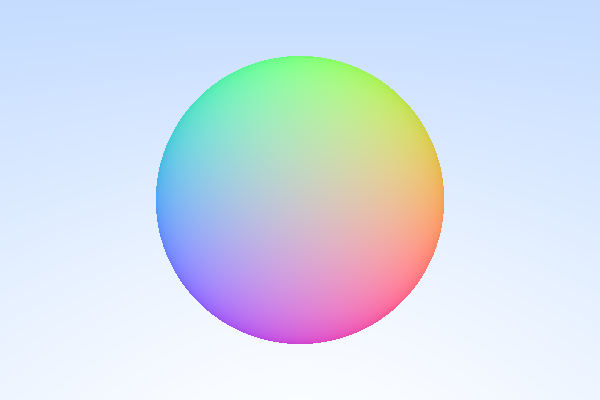
\includegraphics[width=0.7\textwidth]{first_image.png}  
\caption{First rendered scene with a single sphere.}  
\label{fig:first-rendered-scene}  
\end{figure}  

\subsection{d. Blinn-Phong Shading}  
\label{sec:blinn-phong-shading}

Blinn-Phong shading provides realistic lighting effects by combining ambient, diffuse, and specular components.

\noindent\textbf{Implementation:}  
\begin{itemize}
    \item Developed a `BlinnPhongMaterial` class extending the base `Material` class for shading calculations.  
    \item Ambient component: constant colour added to the surface.  
    \item Diffuse component: dot product between surface normal and light direction.  
    \item Specular component: based on the angle between the half-vector (average of view and light directions) and surface normal, raised to a shininess factor.  
    \item Supported multiple light sources by accumulating their contributions.  
    \item Replaced basic shading in the rendering loop with material-based shading at intersections.  
\end{itemize}

\noindent\textbf{Evaluation:}  
The first render using Blinn-Phong shading featured a red sphere at \((0, 0, -1)\) (radius \(0.5\)) and a ground sphere at \((0, -100.5, -1)\) (radius \(100\)). A light source at \((5, 5, -5)\) illuminated the scene. The rendered image showed specular highlights, diffuse shading, and ambient lighting, confirming the model's correct implementation.  

\begin{figure}[H]  
\centering  
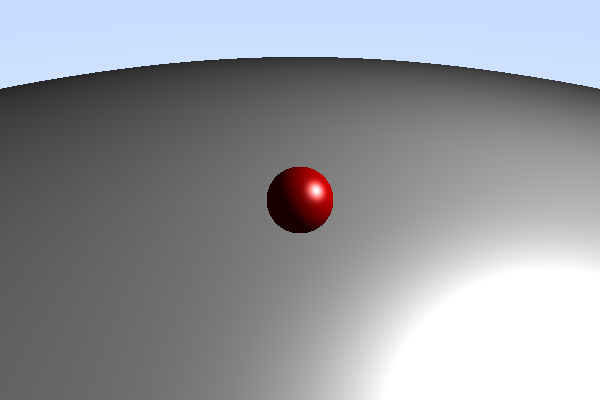
\includegraphics[width=0.7\textwidth]{first_blinn.png}  
\caption{First render using Blinn-Phong shading with one light source.}  
\label{fig:blinn-phong-first}  
\end{figure}

\subsection{e. Shadows}  
\label{sec:shadows}

Shadows enhance realism by accounting for light obstruction caused by objects.

\noindent\textbf{Implementation:}  
\begin{itemize}
    \item Cast shadow rays from hit points to each light source.  
    \item Checked for intersections along shadow rays to determine if a point is in shadow.  
    \item Integrated shadow calculations into the `BlinnPhongMaterial` class, ensuring light contributions are excluded for shadowed points.  
    \item Adjusted diffuse and specular shading based on shadowing.  
\end{itemize}

\noindent\textbf{Evaluation:}  
The implementation was tested with scenes containing multiple objects and a single light source. Two red spheres at \((0, 0, -1)\) and \((-1.2, 0, -1)\), along with a large ground sphere at \((0, -100.5, -1)\), demonstrated accurate shadows on the ground and between objects, significantly improving depth and realism.  

\begin{figure}[H]  
\centering  
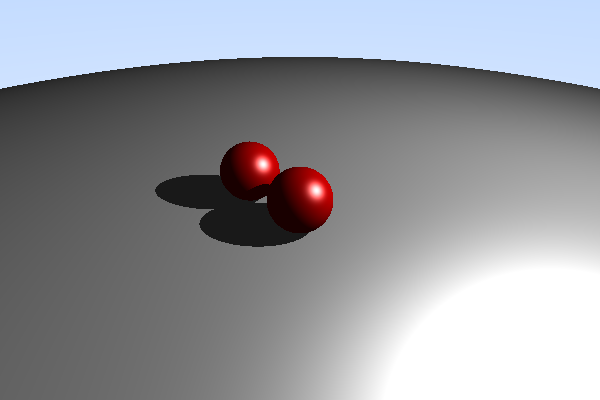
\includegraphics[width=0.7\textwidth]{first_shadow.png}  
\caption{Rendered scene with shadows, showing accurate light obstruction.}  
\label{fig:shadows}  
\end{figure}  

\subsection{f. Tone Mapping}  
\label{sec:tone-mapping}

Tone mapping compresses high dynamic range (HDR) values into a displayable range, enhancing image quality.

\noindent\textbf{Implementation:}  
\begin{itemize}
    \item Created a `ToneMapper` interface and implemented `ReinhardToneMapper` for global tone mapping.  
    \item Applied the formula: \( \text{colour}_{\text{mapped}} = \frac{\text{colour}}{\text{colour} + 1} \).  
    \item Integrated tone mapping into the image save pipeline to process all pixel values before output.  
    \item Added gamma correction for consistent display.  
\end{itemize}

\noindent\textbf{Evaluation:}  
Images with high intensity values were rendered with balanced brightness, avoiding overexposure while preserving detail. Using the same scene as in the shadows evaluation, tone mapping effectively compressed HDR values, particularly improving brightness balance around reflections on the ground sphere.  

\begin{figure}[H]  
\centering  
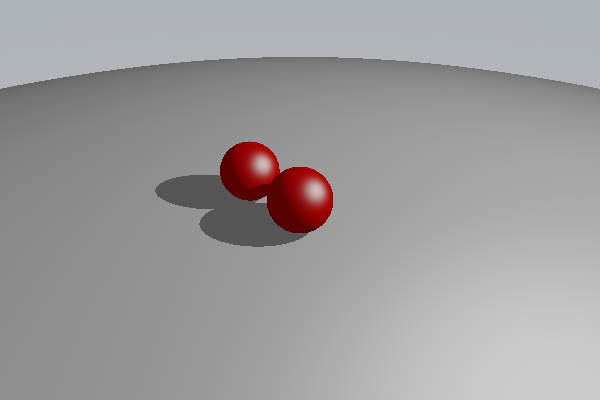
\includegraphics[width=0.7\textwidth]{tone_mapped.png}  
\caption{Rendered scene with tone mapping applied.}  
\label{fig:tone-mapping}  
\end{figure}  

\subsection{g. Reflection}  
\label{sec:reflection}

Reflection simulates mirror-like surfaces, enhancing realism by rendering object and environment reflections.

\noindent\textbf{Implementation:}  
\begin{itemize}
    \item Calculated reflection vectors using \( \text{reflect} = \text{view} - 2 \cdot (\text{view} \cdot \text{normal}) \cdot \text{normal} \).  
    \item Cast secondary rays along reflection vectors to compute reflected colours.  
    \item Combined reflective contributions with Blinn-Phong shading in the rendering pipeline.  
\end{itemize}

\noindent\textbf{Evaluation:}  
A scene featuring a red sphere at \((0, 0, -1)\), a reflective sphere at \((-1.2, 0, -1)\), and a ground sphere was rendered. The reflective sphere accurately mirrored the red sphere and surrounding environment, with reflections behaving correctly at various angles. This confirmed the successful integration of reflection into shading.  

\begin{figure}[H]  
\centering  
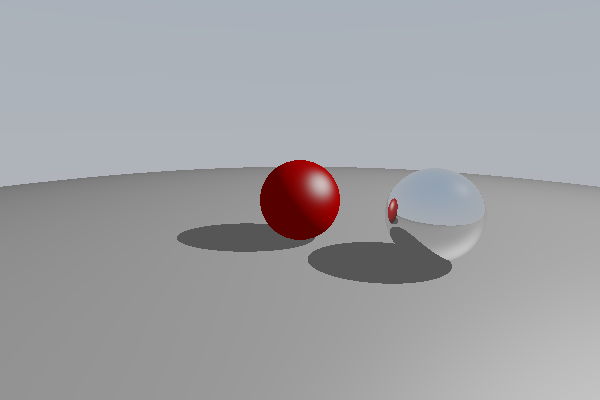
\includegraphics[width=0.7\textwidth]{first_reflection.png}  
\caption{Rendered scene with a reflective sphere.}  
\label{fig:reflection}  
\end{figure}  

\subsection{h. Refraction}  
\label{sec:refraction}

Refraction simulates transparent materials like glass, bending light through objects for added realism.

\noindent\textbf{Implementation:}  
\begin{itemize}
    \item Calculated refraction vectors using Snell's law.  
    \item Applied Fresnel effects with Schlick's approximation for blending reflection and refraction.  
    \item Accounted for total internal reflection (TIR) when the incidence angle exceeded the critical angle.  
    \item Cast secondary rays for refracted light and combined their contributions with Phong shading.  
\end{itemize}

\noindent\textbf{Evaluation:}  
Refraction was tested under various scenarios:  

\begin{itemize}
    \item \textbf{Basic Refraction:} Light bending was validated (Fig.~\ref{fig:basic_refraction}), though without Fresnel effects, visuals were less realistic.  
    \item \textbf{With Fresnel and TIR:} Improved realism with Fresnel effects (angle-dependent reflection) and accurate TIR for critical angles (Fig.~\ref{fig:refraction_fresnel_tir}).  
    \item \textbf{Hollow Glass Sphere:} Demonstrated correct handling of nested IOR transitions with a hollow sphere (Fig.~\ref{fig:hollow_glass_sphere}).  
\end{itemize}

\begin{figure}[h!]  
    \centering  
    \includegraphics[width=0.45\textwidth]{simple_refraction.png}  
    \caption{Basic Refraction (No Fresnel or TIR).}  
    \label{fig:basic_refraction}  
\end{figure}  

\begin{figure}[h!]  
    \centering  
    \includegraphics[width=0.45\textwidth]{fresnel_refraction_with_tir.png}  
    \caption{Refraction with Fresnel Effects and TIR.}  
    \label{fig:refraction_fresnel_tir}  
\end{figure}  

\begin{figure}[h!]  
    \centering  
    \includegraphics[width=0.45\textwidth]{refraction_hollow_air_sphere.png}  
    \caption{Hollow Glass Sphere (Air Interior).}  
    \label{fig:hollow_glass_sphere}  
\end{figure}  

\section{Intermediate Raytracer features}
\label{sec:intermediate-raytracer}
\subsection{a. Textures}  
\label{sec:textures}

Textures add surface details to objects, enabling the application of realistic patterns and images.

\noindent\textbf{Implementation:}  
\begin{itemize}
    \item Developed an abstract `Texture` class with methods to calculate colour based on texture coordinates.  
    \item Implemented `ImageTexture` for mapping PPM texture files:  
    \begin{itemize}
        \item Loaded PPM files, storing pixel data as RGB arrays.  
        \item Used bilinear interpolation for smooth mapping, clamping \( u \) and \( v \) to \([0, 1]\).  
    \end{itemize}  
    \item Supported planar mapping for triangles, cylindrical mapping for cylinders, and spherical mapping for spheres.  
\end{itemize}

\noindent\textbf{Evaluation:}  
Textures were tested on spheres, cylinders, and triangles.

\begin{figure}[h!]  
    \centering  
    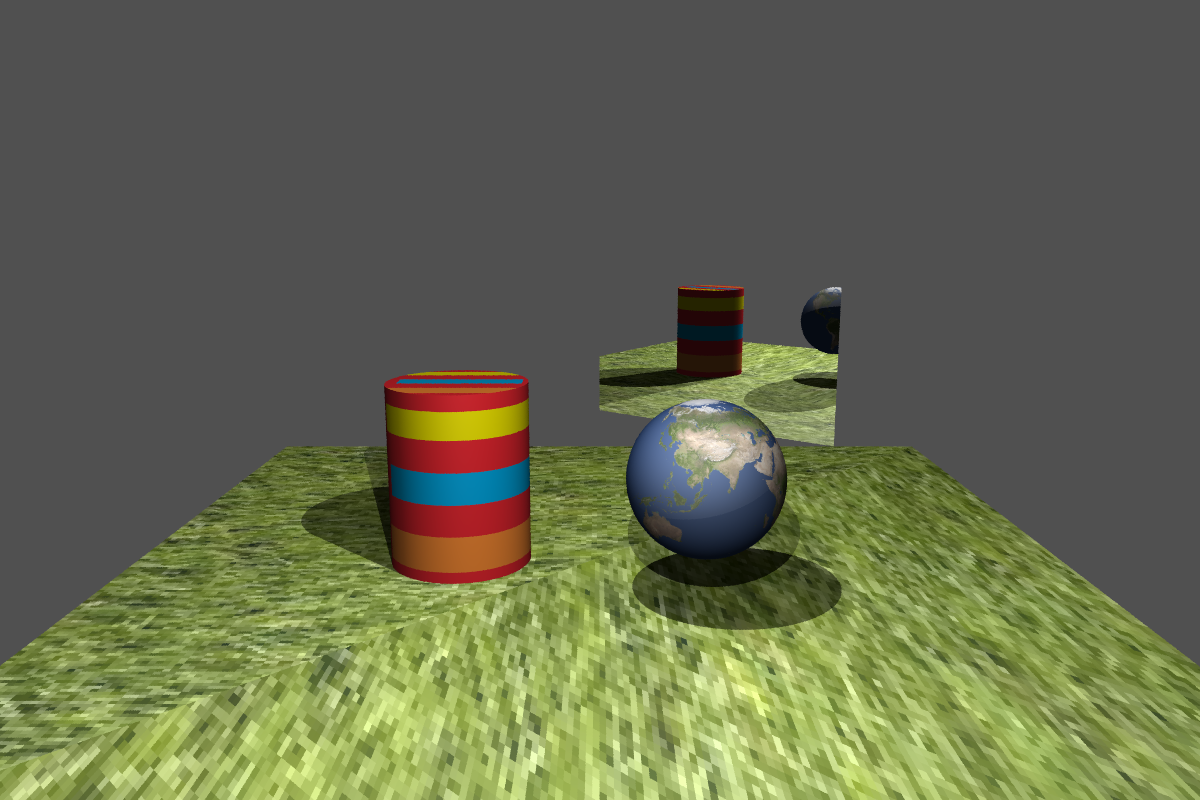
\includegraphics[width=0.75\textwidth]{textures.png}  
    \caption{Rendered scene showcasing texture mapping on spheres, cylinders, and planar surfaces.}  
    \label{fig:textures}  
\end{figure}  

\subsection{b. Acceleration Hierarchy}  
\label{sec:acceleration-hierarchy}
The acceleration hierarchy, implemented using a Bounding Volume Hierarchy, accelerates rendering performance by reducing the number of intersection tests in complex scenes.

\noindent\textbf{Implementation:}  
\begin{itemize}
    \item Created an Axis-Aligned Bounding Box class:  
    \begin{itemize}
        \item Implemented ray-box intersection tests.  
        \item Added methods to compute the surrounding box of two AABBs.  
    \end{itemize}  
    \item Developed a `BVHNode` class to recursively partition the scene into a binary tree:  
    \begin{itemize}
        \item Sorted objects along a random axis for optimal tree construction.  
        \item Leaf nodes stored individual objects, while internal nodes grouped objects with their AABBs.  
        \item Implemented hit logic to traverse the tree, prioritising bounding box checks before object intersections.  
    \end{itemize}  
    \item Updated `Hittable` and derived classes to include a `bounding\_box` method for BVH.  
\end{itemize}

\noindent\textbf{Evaluation:}  
BVH significantly reduced unnecessary intersection tests, improving rendering times. For the scene `scenes/scene\_bvh.json`, performance results are:  

\begin{verbatim}
With BVH:
Total time: 25.5 seconds
Average time per pixel: 0.031875 ms

Without BVH:
Total time: 37.5 seconds
Average time per pixel: 0.046875 ms
\end{verbatim}

The BVH implementation achieved a 32\% reduction in total render time.

% Advanced Raytracer Features
\section{Advanced Raytracer Features}
\label{sec:advanced-raytracer}

\subsection{a. Pixel Sampling}  
\label{sec:pixel-sampling}

Pixel sampling employs multiple techniques to balance image quality and performance.

\noindent\textbf{Implementation:}  
\begin{itemize}
    \item \textbf{Uniform Random Sampling:} Basic Monte Carlo integration with random pixel sampling.  
    \item \textbf{Stratified Sampling:} Divides each pixel into a grid for evenly distributed samples, reducing noise.  
    \item \textbf{Importance Sampling:} Dynamically allocates samples based on luminance importance, focusing on high-variance areas.  
    \item \textbf{Post-Process Filtering:} Applied Gaussian blur and bilateral denoising to further reduce noise.  
\end{itemize}

\noindent\textbf{Evaluation:}  
Uniform sampling established a baseline, while stratified and importance sampling significantly reduced noise and optimised computation. Post-processing filters improved the final image by minimising residual noise.  

\begin{itemize}
    \item \textbf{Uniform Sampling:} Rendered a 1000x1000 image with 500 samples in 243.981 seconds (Fig.~\ref{fig:basic_refraction}).  
    \item \textbf{Importance Sampling:} Rendered the same scene with adaptive sampling (250–10,000 samples), reducing render time by 75\% to 65.723 seconds, albeit with slightly more noise (Fig.~\ref{fig:refraction_fresnel_tir}).  
\end{itemize}

\begin{figure}[h!]  
    \centering  
    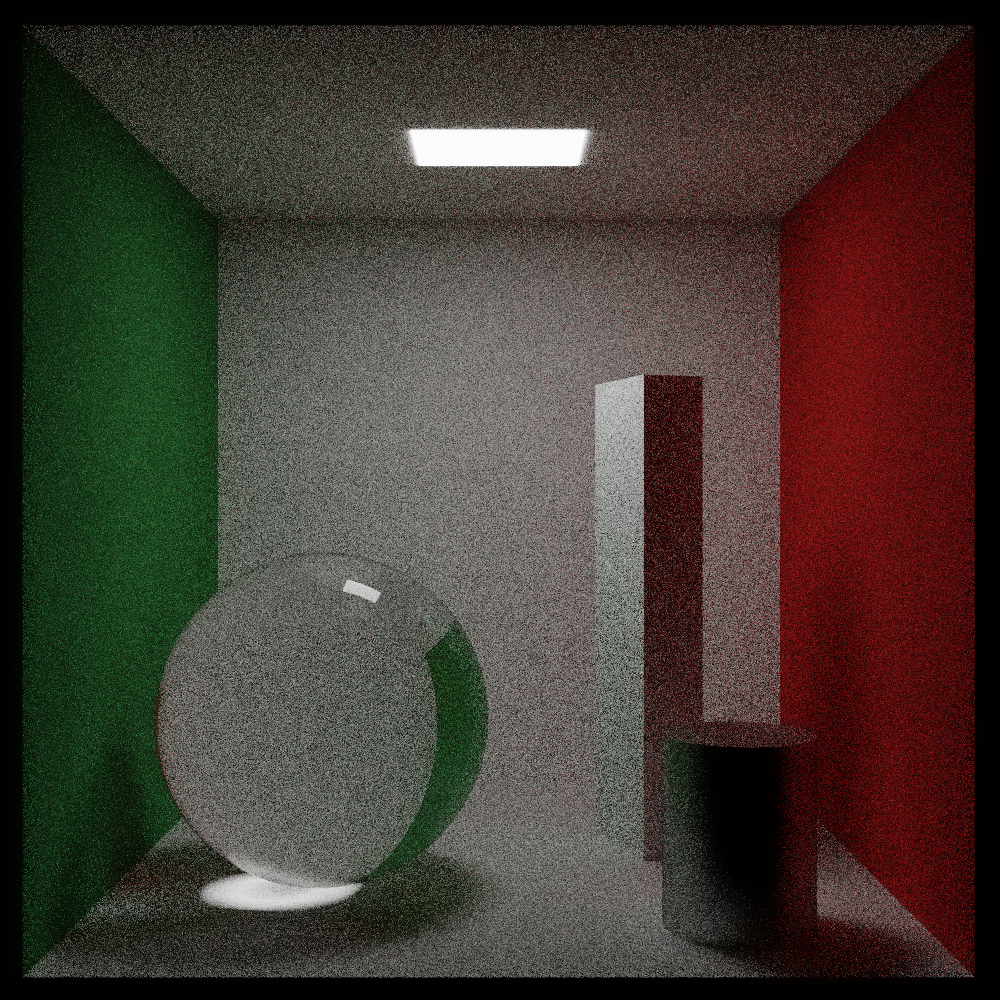
\includegraphics[width=0.45\textwidth]{uniform 500.png}  
    \caption{Uniform Sampling Render}  
    \label{fig:basic_refraction}  
\end{figure}

\begin{figure}[h!]  
    \centering  
    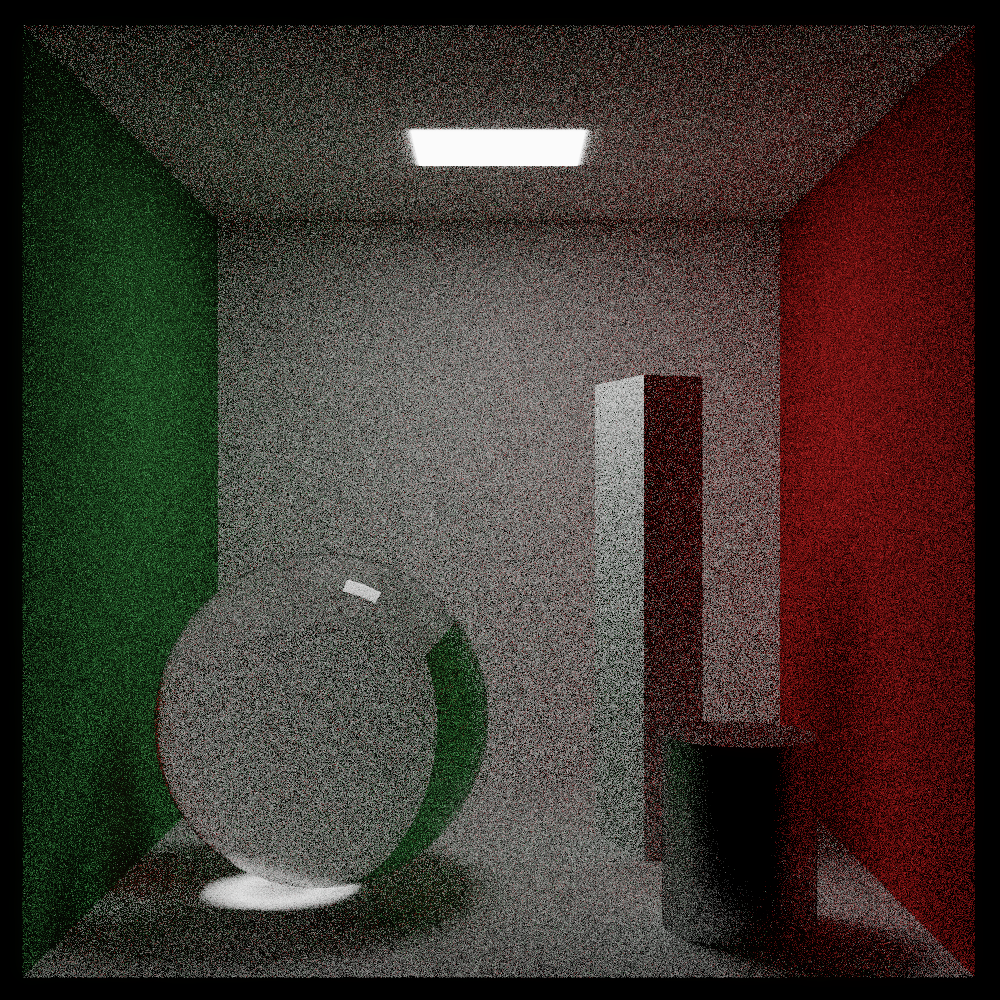
\includegraphics[width=0.45\textwidth]{importance sampling.png}  
    \caption{Importance Sampling Render}  
    \label{fig:refraction_fresnel_tir}  
\end{figure}

\subsection{b. Lens Sampling}
\label{sec:lens-sampling}

Lens sampling simulates depth of field by modelling the camera lens as an aperture, where rays are traced through different parts of the lens. This creates realistic blurring for objects outside the focus distance, mimicking real cameras.

\noindent\textbf{Implementation:}
\begin{itemize} 
\item Extended the \texttt{Camera} class to include lens sampling for depth of field:
    \begin{itemize} 
        \item Introduced a lens\_radius variable, calculated from the aperture size.
        \item Implemented random\_in\_unit\_disk method to sample random points on a unit disk, scaled by the lens\_radius.
    \end{itemize}
\item Modified Camera::get\_ray:
    \begin{itemize} \item Offset the ray origin using sampled points on the lens aperture:
    \texttt{offset = u * rd.x + v * rd.y; ray\_origin = origin + offset}.
    \item Adjusted the ray direction to point to the focus plane:
    \texttt{direction = target - ray\_origin}.
    \end{itemize}
\end{itemize}

\noindent\textbf{Evaluation:}
Depth of field was tested in scene/path\_dof.json with an aperture of 0.6 and focus distance of 6.0. The centre cube remained sharp, while objects outside the focus distance blurred realistically. Fig.~\ref{fig:lens_sampling} demonstrates the accurate depth of field effect.

\begin{figure}[h!]
\centering
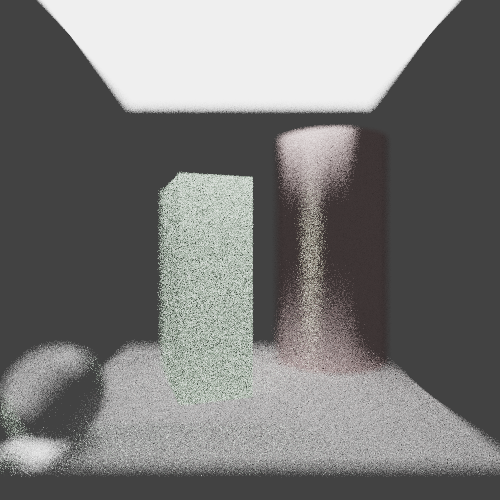
\includegraphics[width=0.5\textwidth]{dof.png}
\caption{Depth of field effect using lens sampling (aperture = 0.6, focus distance = 6.0).}
\label{fig:lens_sampling}
\end{figure}

\subsection{c. BRDF Sampling}  
\label{sec:brdf-sampling}

BRDF sampling models how light interacts with surfaces, enabling realistic simulation of direct and indirect lighting.

\noindent\textbf{Implementation:}  
\begin{itemize}
    \item Implemented the \texttt{brdf} function for each material:  
    \begin{itemize}
        \item \textit{Diffuse}: Used Lambertian BRDF, returning \(\frac{m\_albedo}{\pi}\) for perfect diffuse reflection.  
        \item \textit{Metal}: Calculated specular reflection using a microfacet model with roughness and albedo parameters.  
        \item \textit{Dielectric/Emissive}: BRDF not applied to these materials.  
    \end{itemize}
    \item Incorporated BRDF sampling in \texttt{Pathtracer::trace}:  
    \begin{itemize}
        \item \textit{Direct Lighting}: Sampled light sources, checked for shadows, and computed light contributions using the material's BRDF.  
        \item \textit{Indirect Lighting}: Generated scattered rays using the BRDF's probability distribution and recursively traced rays for indirect contributions, weighted by BRDF values and adjusted for the PDF.  
    \end{itemize}  
    \item Implemented Russian Roulette termination to limit recursion depth based on throughput.  
    \item Used importance sampling to favour high-BRDF-value directions, reducing noise and improving convergence.  
\end{itemize}

\noindent\textbf{Evaluation:}  
BRDF sampling accurately represented material behaviours:  
\begin{itemize}
    \item Diffuse surfaces displayed soft shading and correct light scattering.  
    \item Metallic surfaces showed realistic specular reflections.  
    \item Balanced integration of direct and indirect lighting produced natural shadows and illumination.  
\end{itemize}  

The effects were tested in \texttt{scene/cornell\_box.json}, which includes all material types.

\subsection{d. Light Sampling}  
\label{sec:light-sampling}

Light sampling calculates direct illumination by evaluating contributions from light sources, including shadows and attenuation.

\noindent\textbf{Implementation:}  
\begin{itemize}
    \item Sampled each light by generating direction vectors from the intersection point to the light source.  
    \item Computed light intensity using the inverse square law for attenuation based on distance.  
    \item Cast shadow rays to detect occlusions and determine if light contributes to the surface.  
    \item For unblocked lights, calculated direct lighting as:  
    \[
    \text{Light Contribution} = (\text{attenuated intensity}) \cdot (\text{BRDF value}) \cdot \cos(\text{angle between light direction and surface normal})
    \]
    \item Integrated light sampling within the direct lighting component of the path tracing algorithm for accurate representation of direct illumination.  
\end{itemize}

\noindent\textbf{Evaluation:}  
Light sampling was validated in \texttt{scene/cornell\_box.json}, demonstrating accurate direct illumination, including shadows and realistic light attenuation.  

\section{Conclusion}
\label{sec:conclusion}

The final Cornell box scene was rendered at a resolution of 1000x1000 with a minimum of 500 samples and a maximum of 10000 samples per pixel. Gaussian blur and denoising were also applied to improve render quality. The result is shown in Fig.~\ref{fig:features_combined}.

\begin{figure}[h!]
    \centering
    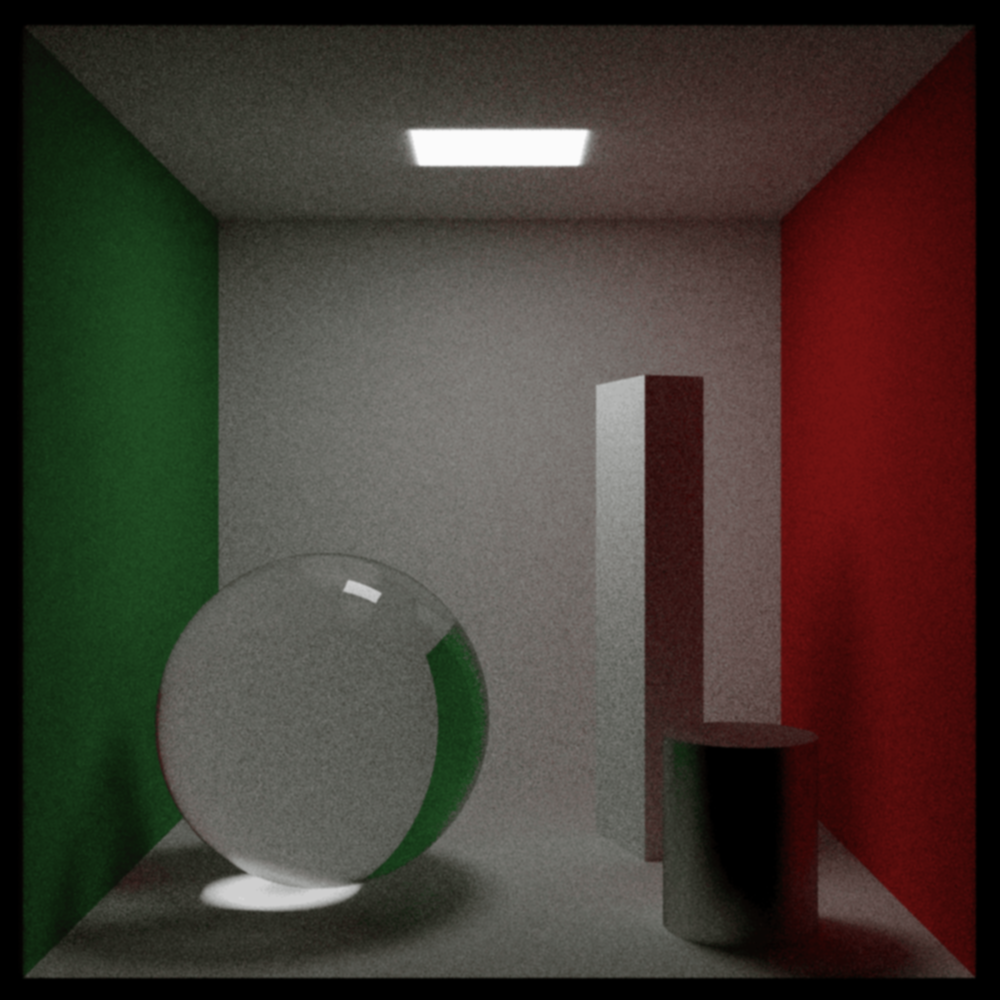
\includegraphics[width=0.45\textwidth]{1000x1000.png}
    \caption{Final render with all features combined.}
    \label{fig:features_combined}
\end{figure}
\end{document}
